\chapter{Excitación de iones por impacto de electrones}

%=======================================================================
\section{Introducción}
\label{sec:intro}

%=======================================================================
\section{Descripción del blanco}

It is well established that highly accurate target descriptions are of
great importance to solve collisional problems with the close-coupling
expansion method~\cite{Bartschat:04,Zatsarinny:16,Ballance:03}. 
However, not only the determination of an adequate atomic structure but 
also the correct description of the collision requires expertise and 
significant computational resources. 

In general, the wavefunction of the target is expressed using the
configuration interaction (CI) method, i.e.,
\begin{equation*}
\Psi_i(\mathbf{r}) =
\sum_j^{N} c_{ji} \, \Phi_j(\mathbf{r})\,,
\end{equation*}
where $N$ is the number of relevant electronic configurations within
the configuration interaction approach and $\Phi_j$ are the wave
functions corresponding to each configuration.
Often, the electronic wave functions are obtained by solving the 
radial part of the one-electron Schrodinger equation with an analytic
potential, 
\begin{equation*}
\left[ \frac{1}{2} \frac{d^2}{dr^2} - \frac{l(l+1)}{2r^2} 
 + V_{nl}^{\mbox{\scriptsize eff}}(\lambda_{nl},r)
 + E_{nl} \right] P_{nl}(r)=0\,,
\end{equation*}
where $V_{nl}^{\mbox{\scriptsize eff}}$ is a radial model potential 
containing the corresponding scaling parameter from the set 
$\boldsymbol\lambda=\{\lambda_{1s},\cdots,\lambda_{nl}\}$. The accuracy 
of the target structure calculations is improved by incrementing the 
number of configurations in the CI, which in turn increases the number 
of parameters to be varied. However, there is neither a systematic nor a 
logical prescription for this procedure.

\begin{figure}[t]
\centering
\includegraphics[width=\textwidth]{figures/rmatrix/example_PS.eps}
\caption{Dependencia de la sección eficaz de excitación por impacto de
electrón con las configuraciones electrónicas incluidas en el CI 
(izquierda) y los pseudoestados (derecha) para la transición dipolar 
prohibida $2s^2\,^1S \rightarrow 2s3s\,^1S$ de Be.}
\end{figure}

\begin{figure}
\centering
\begin{tikzpicture}[remember picture] 
  \node[process] (defcfg) 
              {Definición de configuraciones};
  \node[process] (space) at (defcfg) [xshift=0cm,yshift=-2cm]
              {Definición de espacio};
  \node[process] (var) at (space) [xshift=0cm,yshift=-2cm]
              {Variación de parámetros};
  \node[process] (diag) at (var) [xshift=-2.4cm,yshift=-2.3cm]
              {Diagonalización};
  \node[process] (costo) at (var) [xshift=2.4cm,yshift=-2.3cm]
              {Cálculo de costo};
  \node[decision] (converge) at (costo) [xshift=3.8cm,yshift=0cm] 
              {¿Convergió?};
  \node[process, fill=blue!20] (rmatrix) at (var) [xshift=0cm,yshift=-5cm] 
            {Problema colisional};
  \node[process, fill=blue!20] (rate) at (rmatrix) [xshift=0cm,yshift=-2cm] 
            {Rate Coefficients};
% arrows
  \draw [arrow] 
              (defcfg) -- (space);
  \draw [arrow] 
              (space) -- (var);
  \draw [arrow, bend right=33] 
              (var.west) 
              to ([xshift=-0.5cm,yshift=0cm]{diag.north});
  \draw [arrow, bend right=53] 
              ([xshift=-0.25cm,yshift=0cm]{diag.south}) 
              to ([xshift=0.25cm,yshift=0cm]{costo.south});
  \draw [arrow, bend right=33] 
              ([xshift=0.5cm,yshift=0cm]{costo.north}) 
              to (var.east);
  \draw [arrow, dashed] 
              (costo) -- (converge);
  \draw [arrow, dashed] 
              (converge) |- (space.east) node [near start,left] {No};
  \draw [arrow, dashed] 
              (converge) |- (rmatrix.east)  node [near start,right] {Sí};
  \draw [arrow] 
              (rmatrix) -- (rate);
  \draw [arrow, dashed] 
              (rate.west) -- +(-2.75,0)  
              node [midway,above] {Incorrecto} 
              |- (defcfg.west) ;
\end{tikzpicture}
\caption{Diagrama del cálculo del problema colisional ion-electrón.}
\end{figure}

\newpage
%======================================================================
\section{Optimización bayesiana: procesos gaussianos}
\label{sec:gaussianprocess}


\begin{figure}[H]
\centering
 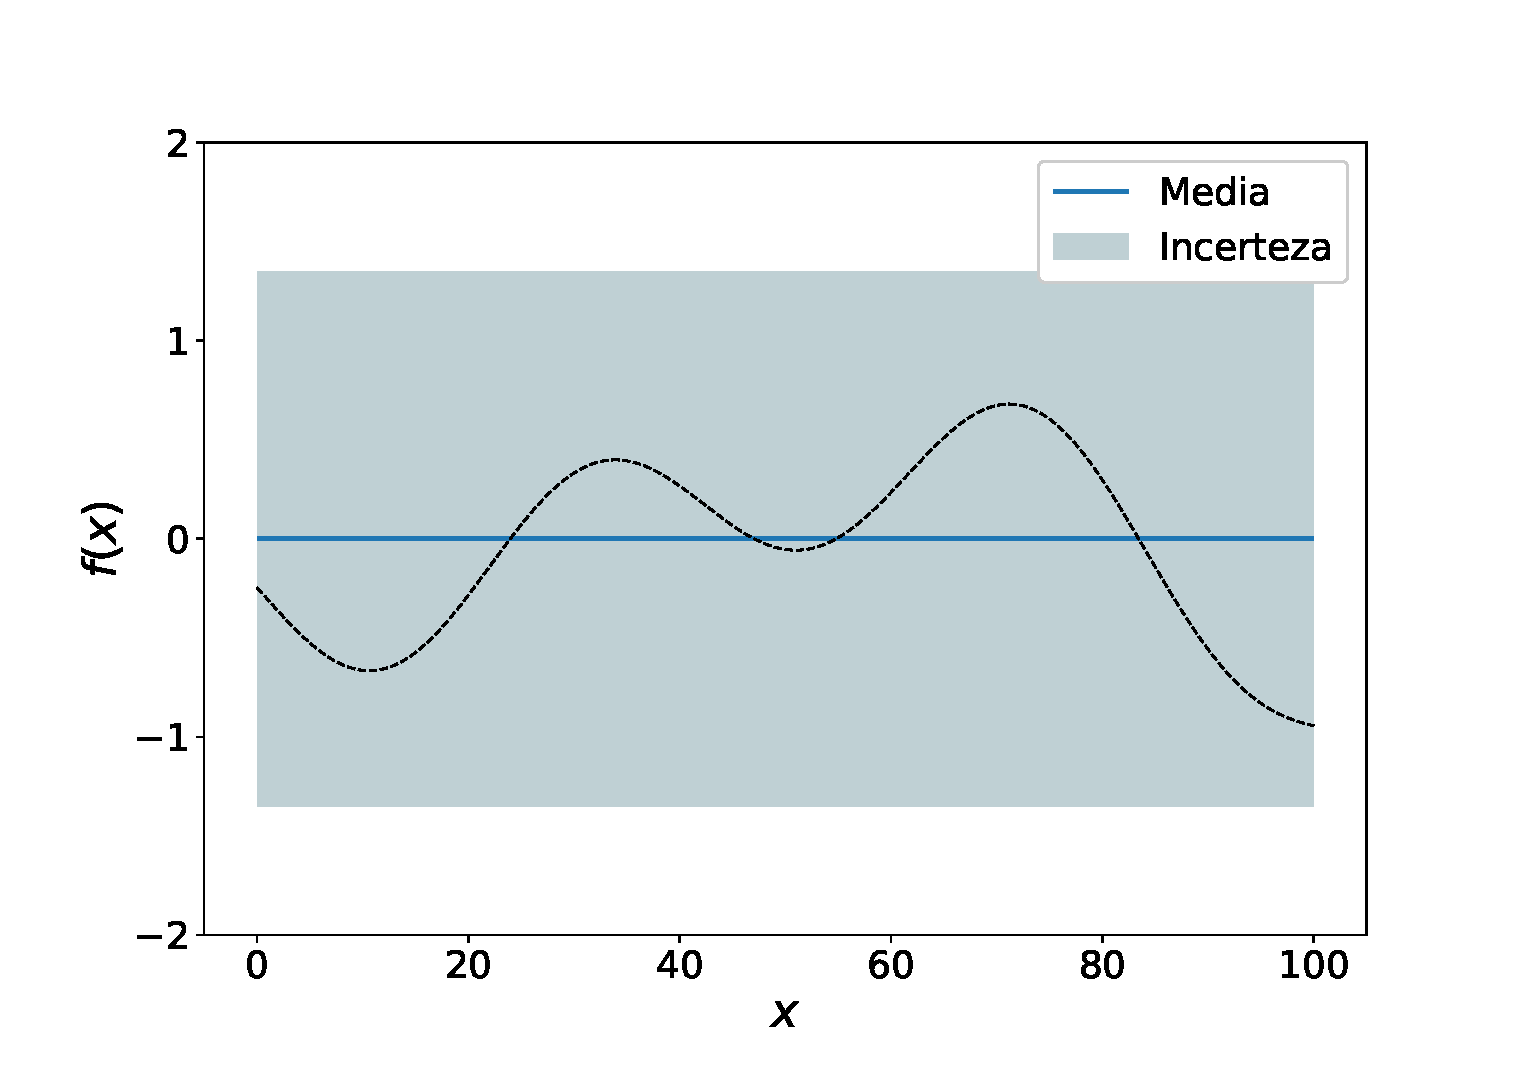
\includegraphics[width=0.31\textwidth]{figures/gp/funcion.eps} 
 \includegraphics[width=0.31\textwidth]{figures/gp/func_acq.eps} 
 \includegraphics[width=0.31\textwidth]{figures/gp/eval1.eps} \\
  \includegraphics[width=0.31\textwidth]{figures/gp/eval2.eps}
  \includegraphics[width=0.31\textwidth]{figures/gp/eval3.eps}
  \includegraphics[width=0.31\textwidth]{figures/gp/eval4.eps} \\
  \includegraphics[width=0.31\textwidth]{figures/gp/eval5.eps}
  \includegraphics[width=0.31\textwidth]{figures/gp/eval6.eps}
  \includegraphics[width=0.31\textwidth]{figures/gp/eval7.eps} 
\end{figure}


\newpage
%=======================================================================
\section{Resultados}


\begin{equation}
J = \sum_{nl} \left|\frac{\widetilde{E}_{nl}(\boldsymbol{\lambda}) 
- E_{nl}}{E_{nl}} \right|
\end{equation}

\begin{table}
\centering
\begin{tabular}{|cc|ccccc|}
\hline 
No & Término      & NIST & Sin opt. & BO $3l$ & BO $4l$ & BO $\bar{5l}$ \\
\hline 
\hline 
1 & $2s^2\,^1S$   & 0.0000 & 0.0000 & 0.0000 & 0.0000 & 0.0000 \\
2 & $2s2p\,^3P^*$ & 0.2003 & 0.2040 & 0.1996 & 0.1989 & 0.1977 \\
3 & $2s2p\,^1P^*$ & 0.3879 & 0.4225 & 0.4079 & 0.3953 & 0.4007 \\
4 & $2s3s\,^3S$   & 0.4746 & 0.4732 & 0.4749 & 0.4744 & 0.4765 \\
5 & $2s3s\,^1S$   & 0.4983 & 0.5016 & 0.4962 & 0.5005 & 0.5002 \\
6 & $2p^2\,^1D$   & 0.5184 & 0.6598 & 0.5203 & 0.5183 & 0.5165 \\
7 & $2s3p\,^3P^*$ & 0.5368 & 0.5376 & 0.5373 & 0.5353 & 0.5353 \\
8 & $2p^2\,^3P$   & 0.5440 & 0.5595 & 0.5442 & 0.5501 & 0.5466 \\
9 & $2s3p\,^1P^*$ & 0.5485 & 0.5574 & 0.5569 & 0.5478 & 0.5498 \\
10 & $2s3d\,^3D$  & 0.5655 & 0.5665 & 0.5582 & 0.5653 & 0.5642 \\
11 & $2s3d\,^1D$  & 0.5871 & 0.5322 & 0.5874 & 0.5892 & 0.5881 \\
\hline
\multicolumn{2}{l}{Energía de ionización} & 0.6852 &  &  &  &  \\ 
\hline
\end{tabular}
\caption{Energía en Rydbergs de los primeros 11 términos de Be relativos 
al término fundamental $2s^2\,^1S$.}
\label{tab:exener}
\end{table}

\begin{table}
\begin{adjustwidth}{-.6in}{-.6in}  
\centering
\begin{tabular}{|lllllllll|} 
\hline 
No & Transición               & Ballance   & Chen       & MCHF       & No opt.    & BO $3l$    & BO $4l$  & BO $5l$ \\
\hline
\hline
1 & $2s2  \,^1S - 2s2p \,^1P$ & $1.37^\dagger$ & $1.38$ & $1.38    $ & $1.32    $ & $1.35    $ & $1.38    $ & $1.31$ \\
2 & $2s2  \,^1S - 2s3p \,^1P$ & $1.12[-2]$ & $9.01[-3]$ & $8.99[-3]$ & $5.70[-2]$ & $6.47[-2]$ & $1.12[-2]$ & $2.14[-2]$ \\
3 & $2s2p \,^3P - 2s3s \,^3S$ & $7.56[-2]$ & $8.23[-2]$ & $8.41[-2]$ & $8.57[-2]$ & $1.28[-1]$ & $7.37[-2]$ & $7.27[-2]$ \\
4 & $2s2p \,^3P - 2s3d \,^3D$ & $2.99[-1]$ & $2.95[-1]$ & $3.00[-1]$ & $2.96[-1]$ & $3.94[-1]$ & $2.70[-1]$ & $2.68[-1]$ \\
5 & $2s2p \,^1P - 2s3s \,^1S$ & $1.20[-1]$ & $1.18[-1]$ & $1.15[-1]$ & $1.62[-1]$ & $1.80[-1]$ & $1.14[-1]$ & $1.27[-1]$ \\
6 & $2s2p \,^1P - 2s3d \,^1D$ & $3.86[-1]$ & $4.10[-1]$ & $3.96[-1]$ & $8.18[-2]$ & $2.57[-1]$ & $3.45[-1]$ & $3.36[-1]$ \\
7 & $2s3s \,^3S - 2s3p \,^3P$ & $1.02$     & $1.13    $ & $1.14    $ & $1.15    $ & $9.11[-1]$ & $1.09    $ & $1.026$ \\
8 & $2s3s \,^1S - 2s3p \,^1P$ & $9.08[-1]$ & $9.58[-1]$ & $9.47[-1]$ & $9.02[-1]$ & $7.56[-1]$ & $9.04[-1]$ & $9.16[-1]$ \\
9 & $2s3p \,^3P - 2s3d \,^3D$ & $4.83[-1]$ & $5.01[-1]$ & $5.14[-1]$ & $4.92[-1]$ & $3.27[-1]$ & $5.06[-1]$ & $4.88[-1]$ \\
10 & $2s3p \,^1P - 2s3d \,^1D$ & $6.91[-1]$ & $6.87[-1]$ & $6.81[-1]$ & $9.26[-2]$ & $7.93[-1]$ & $6.96[-1]$ & $6.67[-1]$ \\
\hline
\multicolumn{2}{c}{$\dagger\,a[b]$ denotes $a\times 10^b$} \\
\end{tabular}
\caption{Oscillator strength de absorción de Be.}
\label{tab:fabs}
\end{adjustwidth}
\end{table}

\begin{figure}
\centering
\includegraphics[width=\textwidth]{figures/rmatrix/erp_ei.eps} 
\caption{Relative error of the first 10 excited terms.}
\label{fig:exener}
\end{figure}

\begin{figure}
\centering
\includegraphics[width=\textwidth]{figures/rmatrix/fabs.eps} 
\caption{Absorption oscillator strength for Be.}
\label{fig:fabs}
\end{figure}



\begin{figure}
\centering
\includegraphics[width=\textwidth]{figures/rmatrix/opt_nl.eps} 
\caption{Secciones eficaces de excitación por impacto de electrón en Be.
Curvas: Dipti \textit{et al.}~\cite{Dipti:19} (discontinua), RMPS sin 
ajuste (punteada); cálculos con optimización bayesiana: 
$3l$ (raya-punto), 
$4l$ (raya-punto-punto), y
$5l$ (continua). 
Símbolos: cálculos CCC de \cite{Fursa:97}.}
\end{figure}

\newpage
%=======================================================================
\section{Conclusiones}
